% The purpose of this chapter is to lay a foundation for understanding the technical choices made in the following chapters.
\chapter{Theory}
\label{chap:theory}
\section{Database management system}

A database is a set of data held in computer storage, often structured for rapid retrieval and modification. A database management system is a system applications can interact with in order to retrieve and modify the data in databases.

As the web has reached a larger percent of the world's population it has grown. Both in numbers and in the professionalism expected by the average user. The number of requests large scale applications experience can in extreme cases reach millions of write operations per second\cite[p.~43]{nosql-ntnu}. Developer expectations of databases has altered to accommodate such use cases. 

\subsection{Distributed database}

Distribution is a paradigm for handling throughput larger than a single server can handle. Distributed databases consists of a network of physically separated computers and a system for maintaining the integrity of the database across multiple computers\cite[p.~4]{ddms}. This enables the database system to distribute the load over each machine, preferably to a computer physically near the client to ensure data localisation. Distributed databases have an advantage in performance and fault tolerance\cite[pp.~12--15]{ddms}.

\subsection{Document-oriented database}

Databases traditionally model relationships between data. These kinds of databases are called relational databases and a relational database management system (RDBMS) is used to enforce certain constraints on the data and the relationships between them. RDBMS are advantageous in ensuring well-formed data and validating queries. However there are problems with this approach for some use cases. NoSQL, of which document-oriented databases are a type, gives up on relational data and its advantages. However one can freely store data whose structure is not known in advance, as is commonly the case in big data. Like distributed databases it also comes with increased performance\cite{cmp-nosql} as there is simply less work for the database to do.

Document-oriented databases associate keys with structured data referred to as documents. The documents are usually stored in a standardised format like XML or JSON\cite[p.~9]{nosql-ntnu}. The document schemes are not constrained, and as such document-oriented databases fall under the NoSQL category.

\section{Continuous Integration}
As has been the truth for a while now, the world wants to become more agile. And as we have been delving deeper and deeper into this new world the need for new tools and methods to achieve this has increased. Continuous Integration was one of the first of these new additions, helping developers prevent integration problems, apply quality control and reduce delivery time. The main goal of CI was to detect and correct errors in the code base early, making them easier to handle. This is done through two key aspects. One is forcing developers to commit their changes daily, this makes the updates small and more manageable. The other key aspect is giving the developers swift feedback, this is done by running automatic tests on the build after committing changes. This new approach made it easier to work incrementally and by extension more agile. Most of the benefits of CI are just side effects, stemming from having to commit daily.

Most of these benefits are based on assumptions in the development world, and there are very few peer-reviewed articles either supporting or disproving these claims. This may be because the claims are hard to test, or there is little interest in the scientific community to answer these questions. Case studies from corporations though, seem to agree with a lot of these claims. But they should not necessarily be viewed as scientific, as they are not peer-reviewed. One of the few scientific articles on the subject though seems to suggest that CI does in fact increase the amount of releases. In fact it appeared that projects using CI had more than double the releases that projects without CI had. 

\begin{displayquote}
One of the more common claims about CI is that it helps
projects release more often, e.g., CloudBees motto is “Deliver
Software Faster” [6]. Over 50% of the respondents from our
survey claimed it was a reason why they use CI. We analyse
our data to see if we can indeed find evidence that would
support this claim.
We found that projects that use CI do indeed release more
often than either (1) the same projects before they used CI
or (2) the projects that do not use CI. In order to compare
across projects and periods, we calculated the release rate
as the number of releases per month. Projects that use CI
average .54 releases per month, while projects that do not
use CI average .24 releases per month. That is more than
double the release rate, and the difference is statistically
significant (Wilcoxon, p < 0.0000)\cite{hilton}.
\end{displayquote}

\section{Continuous Delivery}
Continuous Delivery came as an evolution on Continuous Integration. This new approach is based on making sure the build is deployment-ready at any given time. One would assume this makes the release process longer, as making sure your build is ready for production at any given time requires a bit more work than simply pushing your changes. The research however suggests this is not the case, in fact the following citation seems to suggest continuous deliver has numerous benefits,

\begin{figure}[h!]
  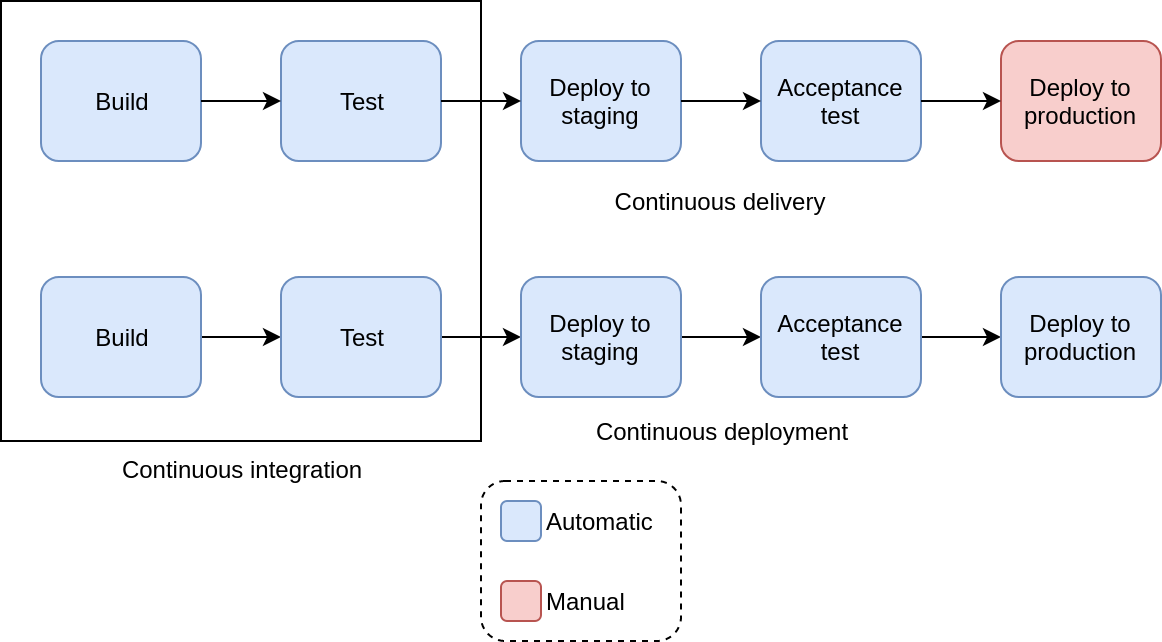
\includegraphics[width=\linewidth,height=\textheight,keepaspectratio]{images/ci_cd_comparison.png}
  \caption{CI/CD comparison}
  \label{fig:CI/CD-comparison}
\end{figure}

\begin{displayquote}
    The practices at the heart of continuous delivery help us achieve several important benefits:
    
    \textbullet ~Faster time to market. It’s not uncommon for the integration and test/fix phase of the traditional phased software delivery lifecycle to consume weeks or even months. When teams work together to automate the build and deployment, environment provisioning, and regression testing processes, developers can incorporate integration and regression testing into their daily work and completely remove these phases. We also avoid the large amounts of re-work that plague the phased approach\cite{continuousdeliveryfaster}.
\end{displayquote}

The advantages of continuous delivery benefit your corporation more than just in throughput and profitability. They increase employee satisfaction, which in and by itself increases worker productivity\cite{happy}.

\begin{displayquote}
    Firms with high-performing IT organisations were twice as likely to exceed their profitability, market share and productivity goals.
    High performers achieved higher levels of both throughput and stability.
    The use of continuous delivery practices including version control, continuous integration, and test automation predicts higher IT performance.
    Culture is measurable and predicts job satisfaction and organisational performance.
    Continuous Delivery measurably reduces both deployment pain and team burnout\cite{forsgren}.
\end{displayquote}

As cited, CD also has other advantages beneficial to organisations.

\section{Reactive programming}
Reactive programming is a paradigm applicable when continuous updates of information is preferred. Data that would traditionally be thought of as single data point is in reactive programming thought of as a stream of points over time. Streams can be transformed and combined to form new streams analogous to how cells in a spreadsheet depend on and update each other. Reactive programming enable elegant propagation of change throughout the domain it is applied to.

\newpage
\section{Security}
While \textit{attack vector} does not have a definition, in the nomenclature of computer security an attack vector usually refers to the path or mechanism by which a system is exploited or otherwise gained unauthorised access to\cite{av1}\cite{av2}\cite{av3}.


The sum of every possible attack vector constructs the \textit{attack surface} of a system. It follows that minimising the attack surface is desirable\cite[p.~1]{as} in a security context. The security community is working on quantitatively measuring the attack surface of a system. Intuitively one might measure the attack surface through the naive methods:

\begin{enumerate}
    \item Counting the number of bugs.
    \item Tracking known vulnerabilities.
\end{enumerate}

However Manadhata et al.\cite{as} suggest (1) is dependent on bug discovery. The process may miss---or have false positive---bugs, and it assigns equal severity to all bugs. (2) does not account for the system's configuration nor does the model capture future attackability.

Manadhata et al. define\cite{as} a method for measuring attack surface that they view as "meaningful and practical". By applying their method a set of attack classes common for CD tools can be built from the type hierarchy seen in figure \ref{fig:th}:

\begin{tabularx}{\textwidth}{| X | c |}
    \hline
    \textbf{Attack class}                  & \textbf{Payoff}\\ \hline \hline
    open\_TCP/UDP-socket                   & .3\\ \hline
    world-accessible\_TCP/UDP-socket       & .4\\ \hline
    open\_unsecured\_env-mgmt              & .6\\ \hline
    open\_secured\_env-mgmt                & .2\\ \hline
    world\_accessible\_secured\_env-mgmt   & .3\\ \hline
    third-party\_credentials               & 1\\ \hline
    world-accessible\_deployment-trigger   & .6\\ \hline
    locally-accessible\_deployment-trigger & .4\\ \hline
\end{tabularx}


\begin{figure}[h]
\makebox[\textwidth][c]{
\begin{tikzpicture}[]
  \begin{scope}
    [tree layout,level distance=10mm,text depth=.1em,text height=.8em, every node/.append style={font=\small}]
    \graph[fresh nodes] {
        all resources <- {
            channel <- {
                TCP or UDP socket <- {
                    world accessible,
                    open
                }
            },
            credentials <- third party trust,
            deployment trigger <- {
                locally accessible,
                world accessible
            },
            httpd module,
            environment management <- {
                unsecured <- {
                    open,
                },
                secured <- {
                    world accessible,
                    open,
                }
            }
        }
    };
  \end{scope}
\end{tikzpicture}
}
\caption{Type hierarchy of the properties in the CD domain}
\medskip
\small
\centering 
Leaf nodes represent attack classes.
\label{fig:th}
\end{figure}

\footnotetext{This figure is based on the type hierarchy example\cite{as} presented in the article by Manadhata et al.}

\textbf{httpd-module}: \begin{displayquote}
"This attack class consists of all resources of type \textit{httpd\_module}. CAN-2003-0789 describes a vulnerability  involving  handling  of  CGI  redirect  in  the \textit{mod\_cgid} module in \textit{apache} which an attacker can exploit to view sensitive information."\footnotemark[2]
\end{displayquote}

\textbf{open\_TCP/UDP-socket}: \begin{displayquote}
"The services  running  on  the system open TCP/UDP sockets and listen for client requests on them. Multiple sockets can be opened by a service and multiple services can share the same socket. This attack class is a subtype of the resource type channel. CVE-2001-0309 describes an attack involving open sockets since the \textit{inetd} daemon does not properly close sockets for internal services such as \textit{daytime} and \textit{echo}, an attacker can cause a denial-of-service attack by opening a series of connections to these services."\footnotemark[2]
\end{displayquote}

\footnotetext[2]{Quote taken from Manadhata et al.\cite{as}}

\textbf{world-accessible\_TCP/UDP-socket}: \begin{displayquote}
This attack class derives from the \textit{open\_TCP/UDP-socket} attack class, however it being accessible by anyone who knows the address increases the risk associated. It opens for the possibility of distributed denial-of-service attacks\cite{ddos}.
\end{displayquote}

\textbf{open\_unsecured\_env-mgmt}: \begin{displayquote}
An integral part of CD is the automatic deployment of programs to environments that run a class of programs. The environments needs to provide an API the CD solution can use to create and restart programs on certain triggers. This API provides attackers with free reign to manipulate programs in the environments if they get access to the network. 
\end{displayquote}

\textbf{open\_secured\_env-mgmt}: \begin{displayquote}
Like \textit{open\_unsecured\_env-mgmt} this class exposes an API for attackers, however the API is secured by TLS certificates, the CD is identified with a certificate signed by the environment. Certificates significantly reduce, but does not eliminate, the attackability of the API. RFC7457\cite{rfc7457} summarises known attacks, as such the possibility of future attacks is present.
\end{displayquote}

\textbf{world\_accessible\_secured\_env-mgmt}: \begin{displayquote}
This attack class is very similar to \textit{open\_secured\_env-mgmt}. Exposing a TLS protected management API to the world is not a big concern as TLS is in widespread use identifying owners of domains by website owners\cite{sslpulse}, and has proven itself not to be an easy target. However it does somewhat increase the associated risk compared to the \textit{open\_secured\_env-mgmt} class.
\end{displayquote}

\textbf{third-party\_credentials}: \begin{displayquote}
Since the CD solution requires access to the environment API an attacker could compromise the CD solution itself and gain access to the environment API through the CD tool. The certificate could also possibly be misused by the third party.
\end{displayquote}

\textbf{world-accessible\_deployment-trigger}: \begin{displayquote}
As part of a larger system CD solution often deploy based on external triggers. An attacker could fake such an external trigger, especially when some external triggers don't support any kind of identification\cite{docker-no-id}
\end{displayquote}

\textbf{locally-accessible\_deployment-trigger}: \begin{displayquote}
Like \textit{world-accessible\_deployment-trigger}, but does not allow external triggers.
\end{displayquote}